\documentclass[11pt]{article}
\usepackage{cite}
\usepackage{graphicx}	
\graphicspath{{img/}}


\begin{document}

% Subject : Symbolic executions technique for finding bugs %
\title{A Survey of\\Symbolic Executions Techniques} % NB: I removed the "for finding bugs" because "bug" is not well-defined and we can clearly state in the introduction why we use symbolic execution.
\author{Hallet Adrien \and Sens Loan}
\date{\today}
\maketitle

  \section*{Abstract}
    % Describe paper's goals and content

  \section{Introduction}
    \subsection{A definition}
      % I tried to explain what is symbolic execution in simple concepts of software engineering
      The first occurences of symbolic execution described the then-new method as a middle ground~\cite{newapproach} between the two most-used method of its time. On one hand, program testing (\emph{e.g.: unit testing}) can not always detect a fault in a program and producing a correct test sample and proving that it indeed is correct is not that easy. On the other hand, program proving can indeed ensure that a program is correct from its entry point to the result but it heavily relys on the proof definitions by the programmer and the formal definition of the problem.\\
      Nowadays, symbolic execution is both described as (part of) the core of many modern techniques to software testing\cite{chopper:icse18} and an effective way to create tests suites with extensive coverage.\cite{threedecadeslater}
    \subsection{The concept}
      The idea behind symbolic execution is to test an algorithm with \emph{symbolic values} rather than concrete values. So instead of using unit testing where a variable is set to a (usually random) value, the symbolic execution maintains a formula that contains all the possible values for the code to reach a particular point in the program. This formula is updated every time the program reaches a branching point. In figure~\ref{fig:symbolicsimple}, we show an example from~\ref{Visser:2004:TIG:1007512.1007526}  of a symbolic execution. Notice how it produces constraints over the variables to explore the algorithm's branching tree.	      % TODO: Adrien <= I'm working on this to warm up :)
      \begin{figure}	
        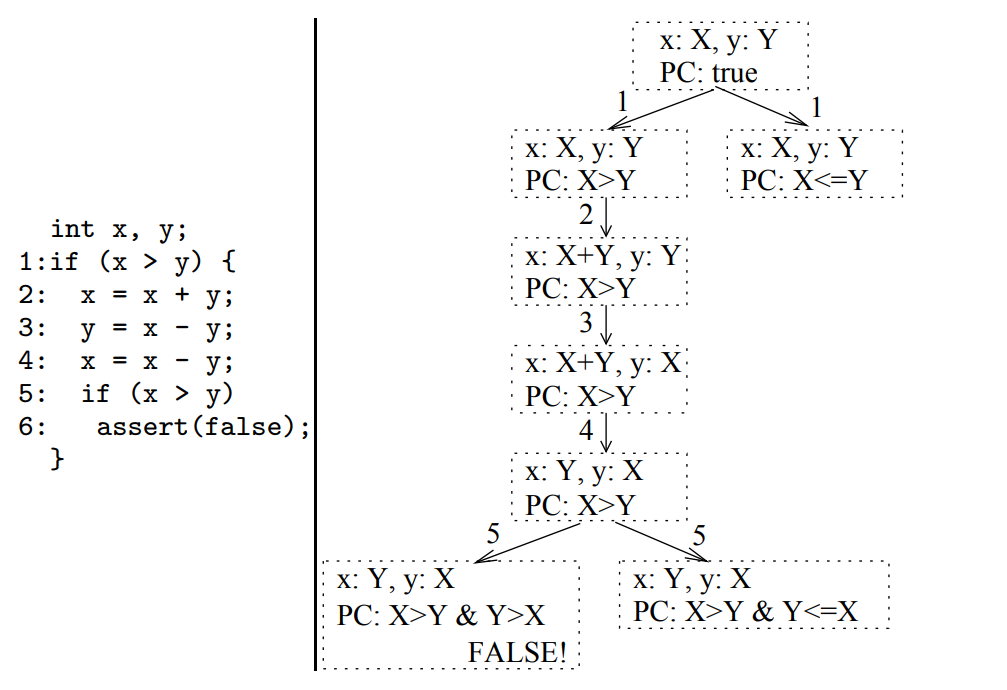
\includegraphics[width=0.5\textwidth]{symbolicsimple}	
        \caption{Swapping two integers and its symbolic execution tree}	
        \label{fig:symbolicsimple}	
      \end{figure}
    % What is symbolic execution and why do we do this survey

  \section{History}
    % Draft the history of symbolic execution, dig any trend up or whatever we can say about it.

  \section{Methods}
    % Begin with anything general to say (if any) then detail methods, could also be useful to compare them (if possible) and/or to say when/why a particular method is being used instead of another.
    % Maybe divide the general techniques and optimisations we can apply to all of them ?
    
    \subsection{Concolic execution}
    \label{subsec:concolicExecution}
    	The name "concolic" is a portmanteau of the words "concrete" and "symbolic", the idea of this testing method is to mix symbolic execution alongside concrete ones.\\
    	
    	This technique concept was first introduced on 2005 \cite{godefroid2005dart}. % The name used wasn't "Concolic" yet but the concept idea was the same
    	Since then the idea was further extended and combined with other testing techniques.

  \section{Tools and languages}
    % Anything general to say bout the content (maybe explain the omnipresence of Microsoft in the market)
    % List tools and language, compare them if possible
    
    % Let DART be first as it is the first used tool to use concolic
    \subsection{\emph{DART} : Directed Automated Random Testing}
    	\emph{DART} is presented as a tool for automatically testing software using concolic testing method (see section \ref{subsec:concolicExecution}). It was introduced in 2005 making it the first the first tool to be created using concolic techniques. \\
    	
    	\subsubsection{Methodology}
	    	\emph{DART} combines three main techniques 	    	\cite{godefroid2005dart} in order to automate unif testing for a particular software :
	    	\begin{enumerate}
	    		\item An automated extraction of the interface of a program with its external environment using static source-code parsing
	    		\item An automatic generation of a test driver for this interface that performs random testing to simulate the most general environment the program can operate in
	    		\item A dynamic analysis of how program behaves under random testing and automatic generation of new test inputs to direct systemically the execution along alternatives program paths
	    	\end{enumerate}
	    	
	    % Add example ? (one on the Godefroy paper, but poorly illustrated) 
	    	
	    \subsubsection{Key strength/originality} 
	    	% TODO [Loan] : need reformulation (copy paste)
	    	The main strength of DART is that testing can be performed completely automatically on any program that compiles – there is no need to write any test driver or harness code.\\
	    	During testing, DART detects standard errors such as program crashes, assertion violations, and non-termination.\\
	    	DART provides an attractive alternative approach to static analyzers, because it is based on high-precision dynamic analysis instead, while being fully automated as static analysis. The main advantage of DART over static analysis is that every execution leading to an error that is found by DART is guaranteed to be sound. Two areas where we expect DART to compete especially well against static analyzers are the detection of interprocedural bugs and of bugs that arise through the use of library functions.\\
	    	
	    	DART is overall complementary to static analysis since it has its own limitations, namely the computational expense of running tests and the sometimes limited effectiveness of dynamic test generation to improve over random testing.
    	

  \section{Conclusions}
    % What can we get from this paper in general
    % Could be pertinent to talk about a kind of "to go further" which could contain adjacent fields of research
    % Could be pertinent to talk about the future of symbolic execution, if there is any new technique being developed, ...


\pagebreak
\bibliography{bibliography}{}
\bibliographystyle{plain}
\end{document}
